% Generic two-column layout. Copy the text of each section into the course template; the numbers come from the saved results.
\documentclass[10pt,twocolumn]{extarticle}
\usepackage[a4paper,margin=0.62in,columnsep=0.22in]{geometry}
\usepackage{times}
\usepackage[T1]{fontenc}
\usepackage{microtype,graphicx,booktabs,amsmath,amssymb}
\usepackage[font=footnotesize,labelfont=bf,skip=2pt]{caption}
\setlength{\parskip}{0pt}\setlength{\parindent}{9pt}
\renewcommand{\dbltopfraction}{0.9}\renewcommand{\dblfloatpagefraction}{0.7}\setlength{\dbltextfloatsep}{6pt plus 2pt minus 2pt}
\setlength{\textfloatsep}{6pt plus 2pt minus 2pt}\setlength{\floatsep}{5pt plus 2pt minus 2pt}\setlength{\intextsep}{5pt plus 2pt minus 2pt}
\usepackage{titlesec}
\titleformat{\section}{\bfseries\large}{\thesection}{0.5em}{}\titlespacing*{\section}{0pt}{7pt}{3pt}
\titleformat{\subsection}{\bfseries\normalsize}{\thesubsection}{0.5em}{}\titlespacing*{\subsection}{0pt}{4pt}{2pt}
\newcommand{\eur}{\,euros}

\begin{document}
\twocolumn[{\begin{center}
{\LARGE\bfseries Seven-Day-Ahead Store Sales Forecasting with Calibrated Prediction Intervals}\\[3pt]
{\normalsize [Your name], ES 678, [Institute] \quad Code: [GitHub URL]}
\end{center}
\begin{abstract}\noindent\small
We forecast daily sales for each of 1,115 Rossmann drugstores seven days ahead, using only information known at that time, and attach an 80\% prediction interval. All splits follow time, hyperparameters are tuned on rolling validation folds, and the April to July 2015 test period is scored once. A LightGBM model reaches a test MAE of 601\eur{} (WAPE 8.4\%) against 2,139\eur{} for last week's value and 1,273\eur{} for the mean of the last four same weekdays. Conformal intervals cover 83.8\% of test days at a nominal 80\%, but only 20 to 24\% on public holidays and Easter, and the model is weak for stores with no history. Planned promotions and calendar features carry most of the signal.
\end{abstract}\vspace{4pt}}]

\begin{figure*}[t]\centering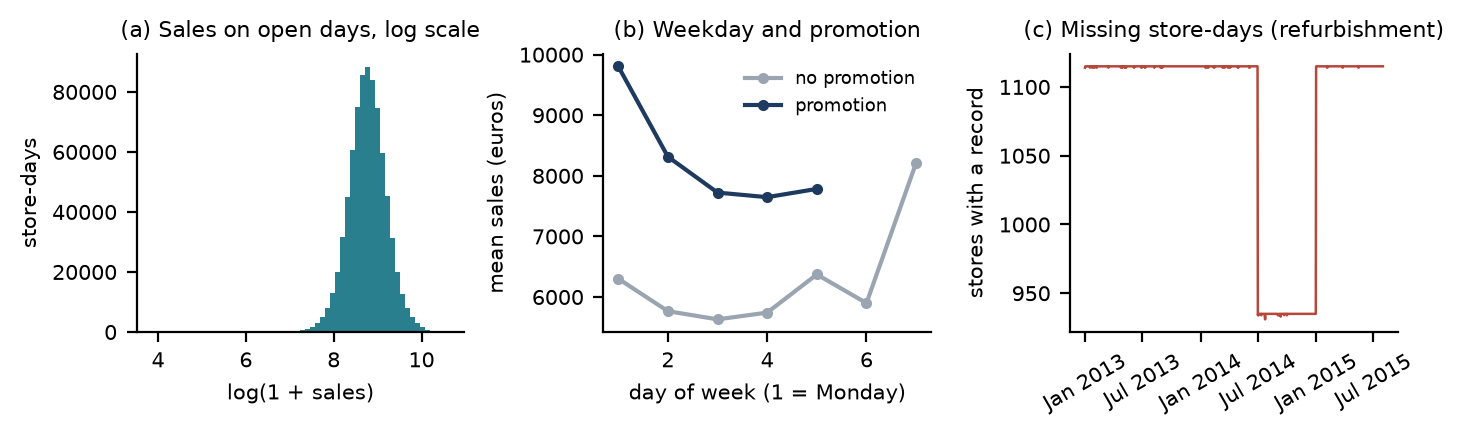
\includegraphics[width=\textwidth]{figures/fig_data.png}
\caption{Data. (a) Sales on open days. (b) Promotions and weekday shift mean sales. (c) 180 stores have no records from July to December 2014.}\label{fig:data}\end{figure*}
\section{Problem}
A store manager must set staffing and stock days ahead. \textbf{Question:} seven days before a trading day, how much will a store sell, and within what range? One row is a store on one open day; the target is daily sales in euros (modelled as $\log(1+\text{sales})$, scored in euros). The forecast is made at the end of day $T-7$ and may use sales up to that day plus facts known in advance: weekday, holidays, planned promotions and store attributes. Same-day customer counts are excluded because they are only known after the day ends. Closed days follow the opening schedule and are not forecast. The model predicts; it does not show that promotions cause sales, because they were not randomised.

\section{Data and preprocessing}
\textbf{Data.} The public Rossmann Store Sales data~\cite{kaggle}: 1,017,209 store-days for 1,115 stores from 1 January 2013 to 31 July 2015, plus one row of attributes per store. Access needs a free Kaggle account and acceptance of the rules; raw files are not redistributed. \textbf{Audit.} 17.0\% of rows are closed days (all with zero sales); 54 open days have zero sales and are rejected; 180 stores have no rows from 1 July to 31 December 2014 (184 days), which matches the refurbishment closures in the competition notes; StateHoliday mixes a number and text codes (0, a, b, c); 354 stores lack a competitor opening date and 544 lack Promo2 fields. Sales are skewed (1.59 raw, $-0.11$ after $\log(1+x)$); the mean on open days is 6,956\eur.

\textbf{Warehouse.} A SQLite star schema (date, store, holiday dimensions; daily sales fact; forecast and audit tables) is loaded one day at a time for 30 days and then in bulk; 31 batches passed 217 reconciliation checks (row and sum totals, keys, duplicates, calendar gaps). Missing days stay missing; they are never turned into zeros.

\textbf{Features and leakage control.} 36 features in five groups: calendar (10), planned promotion (3), store and competition (7), history (15) and a store average (1). History features (same-weekday sales 7, 14, 21, 28 and 364 days back; rolling means, counts and a 28-day trend; promotion and non-promotion averages) are SQL window functions ending exactly seven days before the target, with a minimum number of open days per window. Four tests guard this: features match an independent calculation; multiplying all sales after a cut-off by 10 changes no earlier feature; changing customer counts changes none; and a deliberately planted one-day leak is caught. A shuffled-target check (constant forecast MAE 2,292, shuffled model 2,280, real model 644) shows no label information reaches the model through the pipeline.



\begin{figure*}[t]\centering
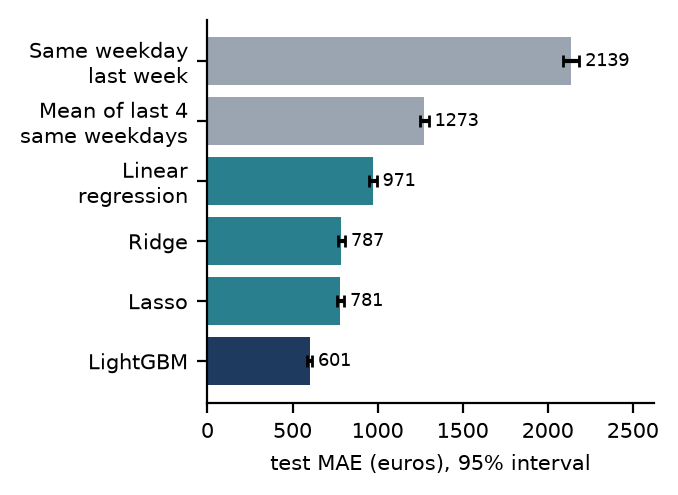
\includegraphics[height=2.35in]{figures/fig_results.png}\hfill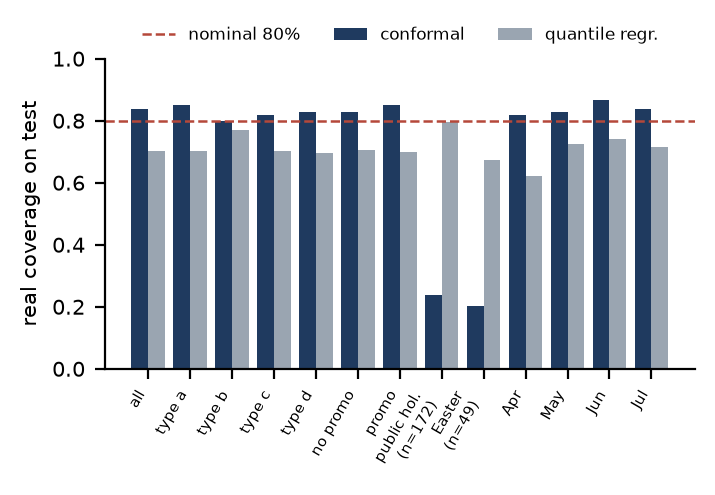
\includegraphics[height=2.35in]{figures/fig_intervals.png}
\caption{Left: test MAE by model with 95\% intervals. Right: real coverage of nominal 80\% intervals overall and by slice; holidays fail.}\label{fig:res}\end{figure*}
\section{Methods and evaluation design}
\textbf{Baselines.} (B0) sales on the same weekday one week earlier; (B1) the mean of the last four same weekdays; (B2) linear regression on promotion, weekday, last week's sales, the 28-day mean and the store average. A one-week-old value is a weak benchmark: on the development folds the value two weeks earlier has a far lower error (MAE 1,328 against 1,990), which fits promotions that alternate between weeks (the promotion flag equals the flag 14 days earlier on 85.5\% of open store-days and the flag 7 days earlier on only 25.1\%), so B1 is the stronger comparison. \textbf{Models.} Ridge and Lasso (squared error plus an L2 or L1 penalty; linear in the features, so sales-scale features are log-transformed to avoid extrapolating the largest stores) and LightGBM~\cite{lgbm} (additive trees on squared error of $\log(1+y)$, which can learn interactions such as promotion by weekday by store type). One global model serves all stores, since each store has under 1,000 days. \textbf{Tuning.} Optuna~\cite{optuna} with 40 trials and 3 seeds per model on a fixed 25\% sample of stores for Lasso and LightGBM; the model is chosen by a rule fixed in advance: the simplest model within one standard error of the best mean fold MAE.

\textbf{Split.} Development data end on 31 March 2015. Five expanding-window folds each validate on 42 days (2 Jun to 13 Jul, 4 Aug to 14 Sep, 6 Oct to 16 Nov, 24 Nov to 4 Jan including Christmas, 16 Feb to 29 Mar). The test period, 1 April to 31 July 2015, was scored once after the choice was committed and tagged. All models are scored on the same rows, those with a seasonal naive forecast (105,267 of 111,421 test rows). \textbf{Metrics.} MAE and WAPE (in euros, not dominated by small stores), MASE~\cite{mase} against the naive forecast, RMSE and $R^2$ (reported with $R^2$ within stores, since most variance is between stores). \textbf{Uncertainty.} 1,000 bootstrap resamples of whole stores, because days within a store are correlated; model differences use the same resamples.

\section{Results}
\begin{table}[t]\centering\footnotesize\setlength{\tabcolsep}{3.5pt}
\caption{Test results, 1 April to 31 July 2015 (euros; 95\% intervals from resampling stores).}\label{tab:res}
\begin{tabular}{lcccc}\toprule
Model & MAE (95\% interval) & WAPE & MASE & $R^2$\\\midrule
Same weekday last week & 2,139 (2,092 to 2,185) & 29.7\% & 1.06 & 0.20\\
Mean of last 4 same weekdays & 1,273 (1,247 to 1,300) & 17.7\% & 0.63 & 0.70\\
Linear regression & 971 (949 to 994) & 13.5\% & 0.48 & 0.80\\
Ridge & 787 (768 to 809) & 10.9\% & 0.39 & 0.86\\
Lasso & 781 (762 to 803) & 10.9\% & 0.39 & 0.86\\
\textbf{LightGBM (chosen)} & \textbf{601 (588 to 615)} & \textbf{8.4\%} & \textbf{0.30} & \textbf{0.92}\\\bottomrule
\end{tabular}\end{table}
LightGBM lowers MAE by 72\% against last week's value (paired difference $-1{,}538$\eur, interval $-1{,}577$ to $-1{,}499$), by 53\% against the four-week mean and by 24\% against Ridge; RMSE is 876\eur, RMSPE 0.116 and $R^2$ within stores 0.77. The development results agree (LightGBM 632\eur{} over five seeds with standard deviation 4.0; Ridge 769\eur), and LightGBM won all five folds, so there is no sign of over-tuning; its 5\% better test score likely reflects training on all development rows. The rule chose LightGBM (best mean fold MAE 642, standard error 73, threshold 715; Ridge at 784 falls outside). The 5.5\% of test rows left out, mostly days after a holiday closure, are easier (MAE 508\eur), so the headline is slightly conservative.



\begin{figure*}[t]\centering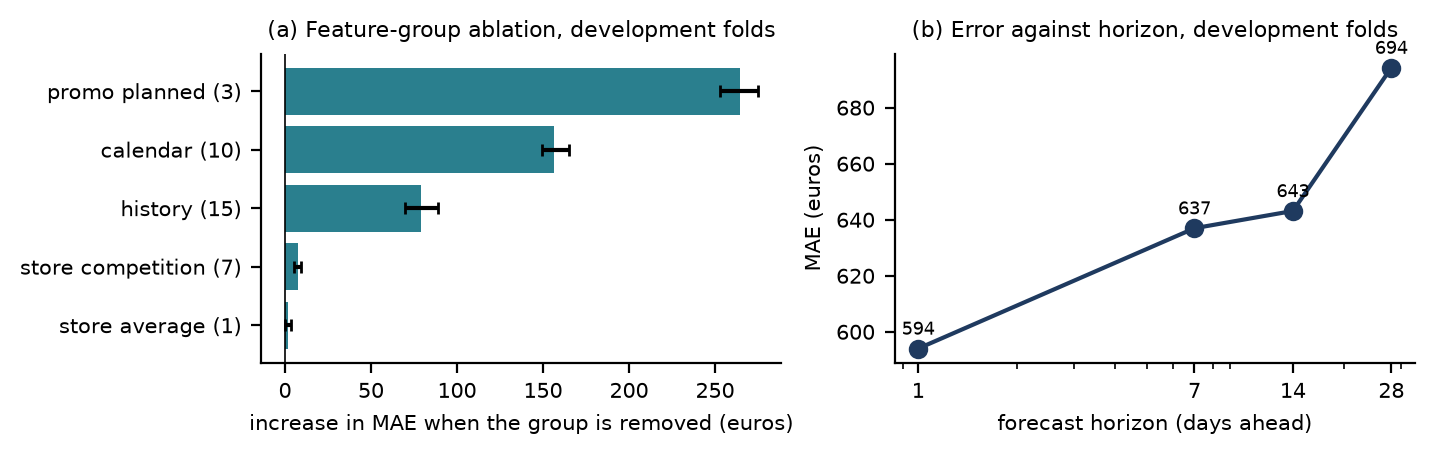
\includegraphics[width=\textwidth]{figures/fig_ablation_horizon.png}
\caption{Left: rise in MAE when a feature group is removed (development folds, half the stores, paired intervals; counts in brackets). Right: MAE against forecast horizon (the vertical axis does not start at zero).}\label{fig:abl}\end{figure*}
\begin{figure*}[t]\centering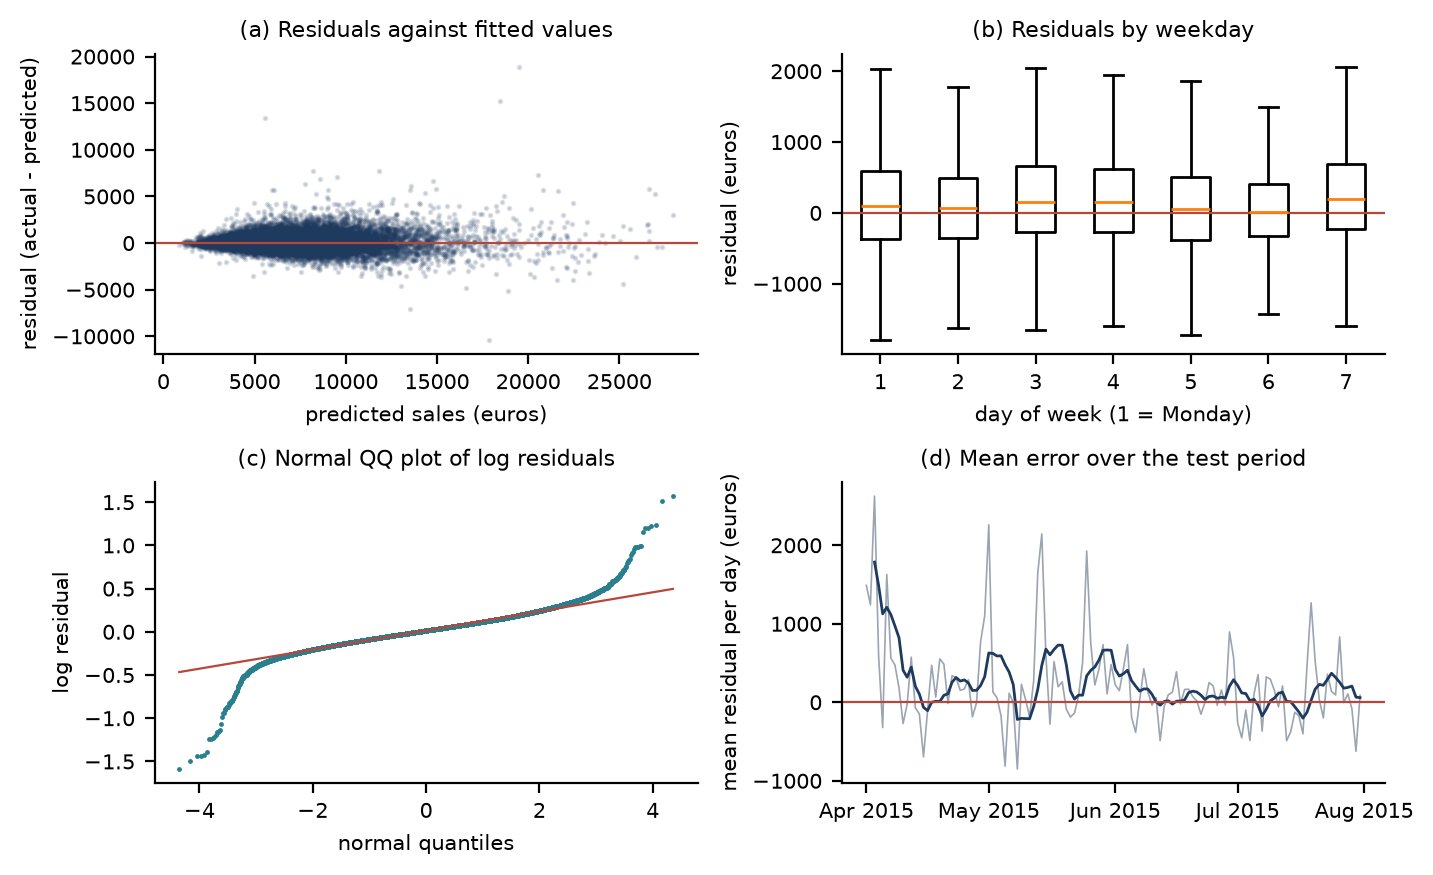
\includegraphics[width=0.7\textwidth]{figures/fig_residuals.png}
\caption{Residual diagnostics for the frozen model on the test period: (a) residuals against fitted values, (b) by weekday, (c) normal QQ plot of log residuals, (d) mean error per day with a 7-day average.}\label{fig:res2}\end{figure*}
\section{Graduate analysis}
\textbf{Uncertainty.} Conformal-style intervals~\cite{conf} use quantiles of out-of-fold log residuals (folds four and five), per store type; LightGBM quantile regression uses the 10th and 90th percentiles. Before the test, the offsets covered 81.6\% of folds one to three. On the test, conformal intervals cover 83.8\% (median width 30\% of the forecast) and quantile regression only 70.2\% (width 21\%), so we use the former. Coverage fails on public holidays (23.8\%, 172 rows) and Easter (20.4\%, 49 rows), where the model under-predicts by about 1,800 to 2,000\eur. Quantile regression, which sees the holiday flag, covers 79.7\% of public holidays but with intervals about 80\% of the forecast wide, so a holiday-aware conformal interval is the obvious fix; we did not tune it on the test. Stocking to a quantile instead of the point forecast cut mean cost per store-day by 24\%, 40\% and 59\% when a shortage costs 3, 5 and 10 times a surplus, with shortages on 24\%, 15\% and 8\% of days (targets 25\%, 17\%, 9\%); sales stand in for demand, which stock-outs censor.



\textbf{Ablation and horizon.} Removing the planned-promotion group raises MAE by 42\% (265\eur; interval 253 to 275), calendar features by 25\%, history by 13\%, store attributes by 1.2\%, and the store average by 0.3\% (interval includes zero). History matters little because static store attributes, such as competition distance, are nearly unique per store and let the model learn store level; this does not carry over to new stores (below). MAE grows slowly with horizon: 594, 637, 643 and 694\eur{} at 1, 7, 14 and 28 days. Adding same-day customers, which cannot be known in advance, cuts MAE by 35\% (628 to 405\eur), which is why it is excluded.

\begin{figure*}[t]\centering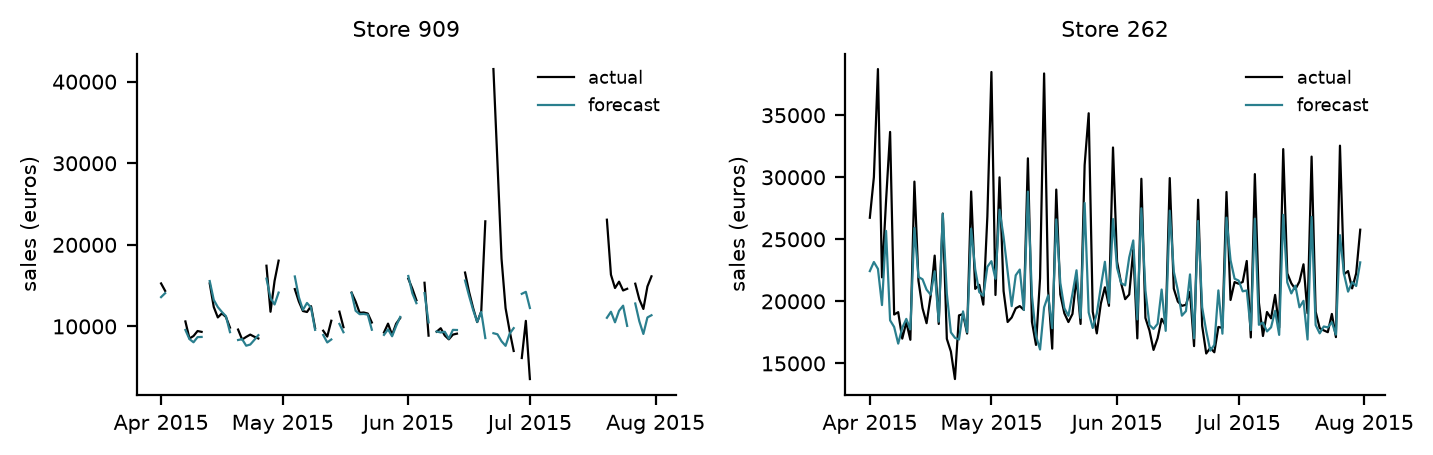
\includegraphics[width=\textwidth]{figures/fig_cases.png}
\caption{Actual and forecast sales for the two stores with the largest MAE. Store 909: a spike of about four times normal sales, then about two weeks with no trading days (lines are broken at gaps). Store 262, one of the largest stores: weekly peaks are followed in timing but understated, and holidays are under-forecast.}\label{fig:cases}\end{figure*}
\textbf{Failure audit.} Relative error is uniform across store types (WAPE 8.2 to 8.8\%) and months (7.8 to 9.1\%); 90\% of store-days are within 17.4\% and store-level WAPE ranges from 7.0\% (10th percentile) to 19.3\% (maximum); store 909 (19.2\%) shows a spike of about four times normal sales in mid-June and then about two weeks with no trading days (Fig.~\ref{fig:cases}), which looks like a temporary closure that no feature could foretell. Public holidays and Easter are the weak slices (WAPE 30\% and 34\%, 0.2\% of rows); several of the largest errors come from store 262, one of the largest stores, on holidays. Easter lay in no validation fold. Mean error is negative from April to June ($-331$, $-201$, $-129$\eur) and near zero in July ($+44$\eur; Fig.~\ref{fig:res2}a, d); the largest weekday bias is on Wednesdays ($-253$\eur). Residuals sit slightly above zero (the model under-predicts by 143\eur{} on average), their spread grows with the forecast, as expected on a log scale (Fig.~\ref{fig:res2}a), and their tails are far heavier than normal (panel c; RMSE over MAE is 1.46 against 1.25 for normal errors), which is why the intervals use empirical quantiles.
Figure~\ref{fig:cases} shows the two worst stores. \textbf{Cold start.} For 112 stores held out entirely and given no history, MAE is 2,557\eur{} (WAPE 35\%), worse than a store-type by weekday median (2,086\eur) and far from the 589\eur{} with history; the model should not be used for new stores without a separate attributes-only approach.




\textbf{Two derivations.} (i) With $\log(1+y)=f(x)+\varepsilon$, a model fitted on the log scale estimates a median-like quantity, while $E[1+y\mid x]=e^{f(x)}E[e^{\varepsilon}]\ge e^{f(x)}$ by Jensen's inequality. Duan's smearing factor~\cite{duan}, the mean of $e^{\hat\varepsilon}$ over development residuals, is 1.019; applying it moved the mean test error from $-143$\eur{} ($-2.0\%$ of sales) to $-7$\eur{} and MAE from 601 to 597\eur. (ii) The pinball loss $\rho_\tau(u)=u(\tau-\mathbf 1[u<0])$ has expected value minimised where $F(q)=\tau$, i.e. at the $\tau$-quantile~\cite{koenker}. With cost $c_u$ per unit short and $c_o$ per unit surplus, expected cost is minimised by stocking the quantile $\tau=c_u/(c_u+c_o)$, which justifies the stocking rule above.

\section{Limitations and conclusion}
One chain, one country and two and a half years: Christmas appears twice in the data and not in the test, Easter once. Promotions were not randomised, so their effect on the forecast is an association. Intervals fail on holidays, sales understate demand when stock runs out, and 5.5\% of test rows were excluded from scoring by the common-rows rule. The test period was used once, after the model choice and settings were committed and tagged \texttt{freeze-before-test}; analysis afterwards read saved predictions only. All dates are fixed in \texttt{config.yaml}, and the repository reproduces every table and figure. Within these limits, a gradient-boosted model with leakage-safe history features forecasts store sales seven days ahead to within about 8\% on average, with intervals that are reliable on ordinary days and unreliable on holidays.

\begin{thebibliography}{9}\footnotesize\setlength{\itemsep}{0pt}\setlength{\parskip}{0pt}
\bibitem{kaggle} Rossmann Store Sales, Kaggle competition, 2015. https://www.kaggle.com/c/rossmann-store-sales
\bibitem{lgbm} G. Ke et al. LightGBM: a highly efficient gradient boosting decision tree. NeurIPS, 2017.
\bibitem{optuna} T. Akiba et al. Optuna: a next-generation hyperparameter optimization framework. KDD, 2019.
\bibitem{mase} R. Hyndman, A. Koehler. Another look at measures of forecast accuracy. Int. J. Forecasting 22(4), 2006.
\bibitem{conf} A. Angelopoulos, S. Bates. A gentle introduction to conformal prediction. arXiv:2107.07511, 2021.
\bibitem{duan} N. Duan. Smearing estimate: a nonparametric retransformation method. JASA 78(383), 1983.
\bibitem{koenker} R. Koenker, G. Bassett. Regression quantiles. Econometrica 46(1), 1978.
\end{thebibliography}
\end{document}
